\documentclass[10pt,a4paper]{article}
\usepackage{pgf,comment}
\usepackage[utf8]{inputenc}
\usepackage{graphics,epsfig}
\usepackage{subcaption}
\usepackage[T1]{fontenc}
\usepackage{float}
\usepackage{url}
\usepackage{srcltx}
\usepackage{hyperref}
\usepackage{amsmath,amsfonts ,amssymb,fancyhdr,setspace,lastpage,comment,graphics, cleveref,natbib}
\usepackage{mathrsfs}
\usepackage{todonotes}
\usepackage[all]{xy}




\DeclareMathOperator{\argmax}{argmax}
\DeclareMathOperator{\id}{id}
\DeclareMathOperator{\Nil}{Nil}
\DeclareMathOperator{\ran}{Ran}
\DeclareMathOperator{\conv}{conv}
\DeclareMathOperator{\cont}{cont}
\DeclareMathOperator{\sign}{sign}
\DeclareMathOperator{\diag}{diag}
\DeclareMathOperator{\colim}{colim}
\DeclareMathOperator{\sing}{sing}
\DeclareMathOperator{\coker}{Coker}
\DeclareMathOperator{\im}{Im}
\DeclareMathOperator{\loc}{loc}
\DeclareMathOperator{\comp}{comp}
\DeclareMathOperator{\findex}{index}
\DeclareMathOperator{\dist}{dist}
\DeclareMathOperator{\op}{op}
\DeclareMathOperator{\spin}{Spin}
\DeclareMathOperator{\pin}{Pin}
\DeclareMathOperator{\SO}{SO}
\DeclareMathOperator{\dom}{Dom}
\DeclareMathOperator{\lip}{Lip}
\DeclareMathOperator{\supp}{supp}
\DeclareMathOperator{\GL}{GL}
\DeclareMathOperator{\Cg}{C^*_{\lambda}(G)}
\DeclareMathOperator{\elset}{\text{ else }}
\DeclareMathOperator{\ift}{\text{ if }}
\DeclareMathOperator{\red}{\text{red}}
\DeclareMathOperator{\Lie}{Lie}
\DeclareMathOperator{\End}{End}
\DeclareMathOperator{\spn}{span}
\DeclareMathOperator{\ind}{Ind}



%i\DeclareMathOperator{\exp}{exp}
\newcommand{\sta}[1]{\text{#1}^{\text{\sout{o}}}}
\newcommand{\de}[2]{\frac{\text{d} #1}{\text{d} #2}}
%\newcommand{\titlez}[1]{\title{#1}\rhead{#1}}
\newcommand{\Lr}{\Leftrightarrow}
\newcommand{\pa}[1]{\left ( #1 \right )}
\newcommand{\nintd}[4]{\int_{#3}^{#4} \!#1 \,\text{d}#2}
\newcommand{\nint}[2]{\int \!#1 \,\text{d}#2}
\newcommand{\refz}[1]{(\ref{#1})}
\newcommand{\dpart}[2]{\frac{\partial #1}{\partial #2}}
\newcommand{\dt}[1]{d{#1}}
\newcommand{\df}[1]{\ensuremath{\mathop{\makebox[0pt]{\hspace{10.5pt}{\(^{\text{-}}\)}}d}} #1}
\newcommand{\abs}[1]{\left | #1 \right |}
\newcommand{\for}[0]{\text{ for }}
\newcommand{\nin}[0]{\notin}
\newcommand{\ol}[0]{\overline}
\newcommand{\comm}[1]{\left [ #1 \right ]}
\newcommand{\F}{\mathcal{F}}
\newcommand{\AS}{\mathfrak{S}}
\newcommand{\osum}{\oplus}
\newcommand{\G}{\mathcal{G}}
\newcommand{\g}{\mathfrak{g}}
\newcommand{\K}{\mathbb{K}}
\newcommand{\V}{\mathcal{V}}
\newcommand{\Adel}{\mathbb{A}}
\newcommand{\De}{\mathbb{D}}
\newcommand{\Cstar}{$C^*~$}
\newcommand{\DO}{\mathfrak{D}}
\newcommand{\E}[0]{\mathcal{E}}
\newcommand{\lin}[0]{\mathcal{L}}
\newcommand{\pd}[0]{$\Psi$DO }
\newcommand{\dlim}{\lim\limits_{\longrightarrow}}
\newcommand{\overbar}[1]{\mkern 1.5mu\overline{\mkern-1.5mu#1\mkern-1.5mu}\mkern 1.5mu}
\newcommand{\exre}[0]{\overbar{\boldsymbolb{R}}}
\newcommand{\lsp}[1]{\mathcal{L}^{ #1 }}
\newcommand{\ip}[2]{\left \langle #1,#2 \right \rangle}
\newcommand{\brak}[1]{\langle #1 \rangle}
\newcommand{\N}[0]{\mathbb{N}}
\newcommand{\C}[0]{\mathbb{C}}
\newcommand{\Z}[0]{\mathbb{Z}}
\newcommand{\T}[0]{\mathcal{T}}
\newcommand{\R}[0]{\mathbb{R}}
\newcommand{\Q}[0]{\mathbb{Q}}
\newcommand{\B}[0]{\mathcal{B}}
\newcommand{\Cl}[0]{\C l}
\newcommand{\M}[0]{\mathfrak{M}}
\newcommand{\tensh}[0]{\hat{\otimes}}
\newcommand{\optens}{\widetilde{\otimes}}
\newcommand{\A}[0]{\mathcal{A}}
\newcommand{\Cu}{\mathcal{O}}
\newcommand{\bwed}[1]{\bigwedge\nolimits^{\!#1}}
\newcommand{\Zred}{\hat{\mathbb{Z}}}
\newcommand{\norm}[1]{\left \Vert #1 \right \Vert }
\newcommand{\D}[0]{\mathscr{D}}
\newcommand{\tens}[0]{\otimes}
\newcommand{\bra}[1]{\langle #1 \rvert}
\newcommand{\ket}[1]{\lvert #1 \rangle}


\renewcommand{\H}{\mathbb{H}}
\renewcommand{\S}[0]{\mathcal{S}}
\renewcommand{\part}[0]{\partial}
\renewcommand{\Re}{\text{Re}}


\let\oldphi\phi \let\phi\varphi \let\varphi\oldphi
\let\oldphi\phi \let\epsilon\varepsilon


%\title{Fast adaptive behavior in a tri-trophic system: Breakdown of the paradox of enrichment}
\title{Emergent population dynamics from behavioral optimization in the water column}
\author{Emil Friis Frølich, Uffe Høgsbro Thygesen}
\date{November 2020}

\begin{document}

\maketitle


\begin{abstract}
  Population dynamics are often modeled without taking behavior into account. This is  in spite of the largest daily feeding times for predators, namely at dawn and dusk, being driven by behavior. The daily pattern stems from the Diel Vertical Migration (DVM) in the aquatic setting and crepuscular behavior in the terrestrial setting. This is usually explained by prey avoiding visual predators, and visual predators seeking to find prey. We develop a game-theoretical model of predator-prey interactions in continuous time and space, finding the Nash equilibrium at every instant. By unifying results for the general resolution of polymatrix games, and a spectral discretization scheme, we can resolve the spatially continuous game nearly instantaneously. Our approach allows a unified model for the slow time-scale of population dynamics, and the fast time-scale of the vertical migration, under seasonal changes. We use the diel vertical migration as a case, examining emergent phenomena from the introduction of the fast dynamics.
  On the behavioral time-scale, we see the emergence of a deep scattering layer from the game dynamics. On the longer time-scale of population dynamics, the introduction of optimal behavior has a strong stabilizing effect, compared to the model without optimal behavior. In a changing seasonal environment, we observe a change in daily migration patterns throughout the seasons, driven by changes in both population and light levels. The framework we propose can easily be adapted to population games in inhomogenous terrestrial environments, and more complex food-webs.
\end{abstract}

\todo[inline]{Abstracted skal nok skrives om til sidst.}

\section{Introduction}
Population dynamics emerges from behavior of the animals; yet many models of population dynamics and ecosystems ignore behavior.  In the past 50 years, game theory has evolved into an invaluable tool for for including animal behavior in ecological models. Game theory gives a theoretical toolkit for understanding observed behavior and making predictions for how behavior will change in response to external changes. Game theory has been used to model a wide variety of situations where an animal needs to make a choice, from habitat choice \citep{krivan1997dynamic, kondoh2003foraging,kvrivan2008ideal}, mating behavior  \citep{rapoport1967exploiter}, and confrontation strategies \citep{smith1973logic}. The game theoretical models have proven successful, with empirical evidence backing up their validity as a model of animal behavior \citep{cooper1989communication,empirical_trait,behavioral_effects}. Specifically, population games where the behavior is adapting instantaneously have emerged as a powerful tool to incorporate behavior in simple population models \citep{Krivan1998,genkai2007macrophyte, cressman2010ideal,pinti2021co, abrams2007role}. The approach used in these models is not scalable to larger number of species or continuous habitats.



Population games often simplified by only considering  one or two trophic levels, \citep{cressman2010ideal, abrams2007role, sadowski2019predator}. This is in spite of e.g. mating behavior being influenced by the risk of predation, \citep{carranza1999red,lima2009predators}, naturally leading to a game with at least three players. Going to games with larger number of players can explain complex phenomena, which cannot be modeled with only two types \citep{pinti2019trophic}. Natural habitats often have continuous fitness gradients \citep{kawecki2004conceptual}, yet population games typically simplify this complex to only a small finite number of patches, \cite{valdovinos2010consequences}. Population models in continuous space with multiple trophic levels or roles are generally hard to examine, as finding Nash equilibria in the resulting games is often prohibitively hard, \citep{empirical_trait,pinti2019trophic}. Resolving the issues of computing Nash equilibria quickly in a continuous setting allows the extension of population games to more realistic models. The question of whether to include behavior in a model or not becomes a question of relevance to the model rather than feasibility.


A critique of game-theoretical models is the assumption that players have perfect information and act in a perfectly rational manner, \citep{jones1999bounded}. Perfect information seems unreasonable, as animals do not have perfect state information \citep{simon1955behavioral}. In addition the minor gain in fitness from the almost-perfect choice to the perfect choice is often outweighed by the higher cognitive or sensorial cost of finding the perfect strategy \citep{simon1956rational, cohen2019bounded}. Though these concerns are well-founded, most models end up incorporating perfect rationality and information anyway. Classical satisficing models of bounded rationality cannot be verified empirically \citep{nonacs1993satisficing}, and with other attempts the \citep{bayesianmodel, thuijsman1995automata} the complexity has prevented the models from being implemented at the population level.



%When introducing uncertainty or bounded rationality, some attemps have been made to incorporate uncertainty in the theory of optimal foraging,

We introduce a method allowing the incorporation of behavior and imperfect decision making in  population games in continuous space and time. The approach we introduce can readily be applied to study multi-species population dynamics emerging from a habitat-choice game in both continuous and discrete habitats. We apply the method to the diel vertical migration, studying the seasonal interplay between population dynamics and behavior. Our model is an extension of the model studied in \citep{verticalmigration} to a population game. Our basic approach is to rephrase a continuous habitat selection game as a single linear complementarity problem, \citep{miller1991copositive}. We incorporate bounded rationality by requiring the strategies solve a diffusion equation, picking the strategy that maximizes the payoff with a given level of noise.
We couple the time scales of population dynamics and behavioral time scales, which allows us to examine how the vertical distribution of predators and prey change throughout the seasons and how this influences the population dynamics. We investigate the length and magnitude of the feeding rates of predators and consumers at throughout the day in spring, summer, and autumn of a single year. We examine how the optimal behavior with noise differs from that without noise, and how noise changes the population dynamics.

%%% Local Variables:
%%% mode: latex
%%% TeX-master: "main"
%%% End:

\section{Method}

%\todo[inline]{Jeg ville gerne se det generelle udbygget lidt og ``kælet for''. }

\subsection{General model and the discrete motivation}
\label{sec:gen_model}
Our general model is that of a population-game \citep{kvrivan2009evolutionary} where the populations can migrate in a continuous habitat on a much faster time-scale than population dynamics \citep{cressman2006migration, abrams2007role}.

To understand the intrinsic coupling of patch-choice models with population dynamics,
consider a Lotka-Volterra model with $M$ patches and $T$ types. Assume the interactions of animals of type $i$ with type $j$ is given by a matrix $A_{ij}$, describing the inter-patch interactions. The intrinsic growth of type of $i$ at patch $k$ is given by $G_{i}(k)$. Assuming that the populations are distributed according to $(p_i)_{i=1}^N$ the population dynamics of type $i$ with total abundance $N_i$ become:
  \begin{equation}
  \dot{N}_i = N_i \sum_{k=1}^M p_i(k) \pa{\sum_{j=1}^T {(A_{ij}N_j) p_j}(k) + G_i(k)} %, ~i\neq
  \label{eq:pop_dyn_lv}
\end{equation}
%\todo[inline]{Udmærket generel formulering - men den skal lige poleres. Hvad med et konstant specifikt vækstled? Beskriver $N$ både antal arter og antal patches? Brug i øvrigt ikke $N$, da det også er abundancen. Brug ikke $A$ for både interaktionsmatricen og fitness. Jeg kan ikke gennemskue detaljerne i notationen ... }
%\todo[inline]{Konstant vækstled tilføjet, patches vs arter ryddet op. }
We define the fitness proxy for an individual by the individual growth rate:
%\todo{Jeg er ikke glad for at kalde en vækstrate for ``fitness''. Du bruger det vist i betydningen ``det der optimeres''. Men fitness defineres normalt som et individs forventede antal efterkommere. Brug evt. ``fitness proxy''.}
of an individual of type $i$ at patch $k$ by $F_i(k)$:
\begin{equation}
  F_i(\phi_i, (N_j \phi_j)_{j \leq T, j \neq i})(k) = p_i(k) \pa{\sum_{j=1}^T {A_{ij}N_j p_j}(k) + G_{i}(k)} %, ~i\neq
  \label{eq:utility_pm}
\end{equation}
If migrations are very fast and the habitat is highly interconnected \citep{abrams2007role, cressman2006migration}, it is reasonable to assume all animals of any type simultaneously seek to find the optimum patch in the sense of seeking $k$ to maximize \Cref{eq:utility_pm}. A population where every individual follows the optimal strategy for patch selection at any instant, that is finding $k$ to maximize \Cref{eq:utility_pm}, cannot be invaded by mutants following other strategies, so it constitutes an evolutionarily stable strategy \citep{kvrivan2009evolutionary}. The approach of using population dynamics determined by \Cref{eq:pop_dyn_lv} with optimal strategies determined by the Nash equilibrium defines a population game, and is a successful approach to coupling optimal behavior with population dynamics \citep{valdovinos2010consequences, mougi2019adaptive, pinti2021co}.

%The ideal free distribution is the resulting distribution  It arises from behavioral optimization in a multi-species Lotka-Volterra model with patches,


The system of utilities in \Cref{eq:utility_pm} can equivalently be interpreted as a polymatrix game \citep{howson1972equilibria}. This interpretation comes if we assume that individuals of type $i$ choose their positions randomly according to the distribution $(p_i)$, instead of having a fixed position $p_i(k)$, i.e. a monomorphic population rather than a polymorphic population. A polymatrix game has so-called polymorphic-monomorphic equivalence \citep{broom2013game}, so an individual of type $j$ cannot determine whether it is playing against a polymorphic population with pure strategies, or a monomorphic population with a mixed strategy. This insight is essential in generalizing to the continuous case, since it highlights that the important factor in \Cref{eq:utility_pm} is the distribution on patches $p_i$.

In nature many habitats are continuous and cannot be described well as discrete patches, so our approach provides a way to resolve population games while keeping the continuous nature of the habitat.

To extend population games to continuous space and facilitate the incorporation of imperfect decision making, we consider a habitat described by an interval $[0,z_0]$. We again assume we have $T$ different types. Define the continuous analogue of the patch distribution $p_i$ by:
\begin{equation}
  K = \{ f \in L^2([0,z_0]) : f \geq 0,~\int f dz = 1\}
  \label{eq:space_of_dists}
\end{equation}
i.e. $K$ is the set of square-integrable probability distributions on $[0,z_0]$. The quantity $N_i \phi_i(z)$ gives the population of type $i$ at $z$. Interactions between animals of type $i$ and $j$ are given by bounded linear operators $U_{ij}: L^2([0,z_0]) \to L^2([0,z_0])$. A bounded linear operator on $L^2([0,z_0])$ can be thought of as an infinite-dimensional matrix. In case the interactions are local, the operators $U_{ij}$ reduce to multiplication by bounded functions, corresponding to diagonal matrices. This consideration explains why we require square-integrability, since we want to be able to consider purely local interactions. As in the finite case, we define the local intrinsic growth by a bounded function $G_i$. Using $G_i$, $K$, and $U_{ij}$ we can define the fitness proxy $F_i$ of an individual of type $i$ playing strategy $\phi_i$ in the continuous setting:
%\todo[inline]{Afhængigt af tidsskriftet bør vi overveje om det med $U$-operatoren skal gøres mere eksplicit.}
\begin{equation}
  F_i(\phi_i, (N_j \phi_j)_{j \leq T, j \neq i}) = \sum_{j=1,j\neq i}^T \int \phi_i(z) (U_{ij}N_j \phi_j)(z) dz + \int \phi_i(z) G_i(z) dz %, ~i\neq j~n_{ij}=1,~i=j~n_{ij} = \frac{1}{2}
  \label{eq:utility}
\end{equation}
The game given by maximizing all $F_i$ with respect to $\phi_i$ is the continuous analogue of a polymatrix game. Since the game again has polymorphic-monomorphic equivalence, the Nash equilibrium for the individual habitat selection game is also given by finding the Nash equilibrium of the game specified by \Cref{eq:utility}.

Modeling the population dynamics, we assume that at every instant the animals are distributed according to the Nash equilibrium of \Cref{eq:utility}. That is, no animal can increase their utility by unilaterally deviating from their strategy. Denoting the Nash equilibrium by $(\phi_i^{*,NE})^T_{i=1}$, the population dynamics are:
\begin{equation}
  \dot{N_i}((\phi_j^{*,NE})_{j=1}^T ) = N_i F_i((\phi_j^{*,NE}, N_j)_{j=1}^N)
\end{equation}

The model we use can theoretically be used for other situations than habitat-choice and population dynamics. As long as the population dynamics can be formulated in way where they are proportional to sums of bilinear payoffs in the strategies, our approach can be used.

%\todo[inline]{Udmærket struktur; skal bare gennemskrives en gang.}
%\todo[inline]{Gennemskrivning i gang; Færdig}


\subsubsection{Noisy strategies}
Our model incorporates that animals are not necessarily perfectly rational: The animal may not be a perfect decision-maker and may choose a slightly sub-optimal habitat, due to imperfect information or limited capacity of information processing, but it can also model errors in our perception of the animal's objectives, or inability to actuate a decision perfectly, for example due to turbulence in the water column. Our model of imperfect rationality is as follows: Say that an animal of type $i$ aims to play the strategy $f_i(\cdot)$, which is a probability density function on $[0,z_0]$. Then our model posits that the animal actually plays a strategy $\phi_i(\cdot ,\sigma)$, which is a smoothed version of $f_i(\cdot)$ obtained by solving the initial value problem
\begin{equation}
  \begin{split}
  \label{eq:density_PDE}
  \partial_s \phi_i &= \frac{1}{2}\partial_z^2 \phi_i \\
  \partial_z \phi_i \mid_{z=0} &= 0 \\
  \partial_z \phi_i \mid_{z = z_0} &= 0 \\
   \phi_i(z,0) &= f_i(z) \quad .
 \end{split}
\end{equation}
on the interval $[0,\sigma]$. Thus, the parameter $\sigma$ determines the degree of smoothing: With $\sigma=0$, the animal is perfectly rational ($\phi_i(z,0)=f_i(z)$) while with $\sigma=\infty$, we have a completely random decisions where $\phi_i(z,\infty)$ is a constant function of $z$, corresponding to a uniform distribution on $[0,z_0]$. Note that $s$ or $\sigma$ are not connected to time; this smoothing takes place instantaneously at each point in time.

Numerically, this smoothing is performed by first determining the fundamental solution to this initial value problem, ignoring boundaries, which is a Gaussian kernel. Then the boundary conditions are implemented using the method of images. Finally, the initial condition is convolved with this kernel.


\subsubsection{Spatial discretization}
In order to calculate the Nash Equilibrium efficiently, and perform numerical integration precisely we discretize the interval $[0,z_0]$ with a spectral scheme based on Legendre polynomials, \citep{kopriva2009implementing}. This allows precise integration and differentation with only relatively few points. Working on a grid with $M$ points, a strategy is a linear combination of normalized hat-functions, where the hat functions are given by:
\begin{align*}
	& \int_{z_{i-1}}^{z_{i+1}} e_i dz = 1 \\
	&e_i(z_{i-1}) = 0,~ e_i(z_{i+1}) = 0
\end{align*}
where the overall strategy becomes:
\begin{align*}
  &\phi_{i} = \sum_{j=1}^M a_{j,i} e_j, \quad i\in \{1,\dots, N\} \\
  &\sum_{j=1}^M a_{j,i} = 1 \quad i\in \{1,\dots, N\}
\end{align*}
The strategy of a player, or type, is fully determined by the $a_i$'s.


When considering non-optimal actors, we need to implement the convolution with $f_Y$, which also assures that the resulting distribution is smooth. An added benefit of incorporating bounded rationality then becomes that our strategy profiles are guaranteed to be smooth, decreasing the number of points needed for exact evaluation of the integrals.


\subsubsection{Finding the Nash Equilibrium}
Finding the Nash Equilibrium in a game in continuous space is usually a hard task, requiring the development of bespoke methods, \citep{verticalmigration, jerome}. The method we use circumvents these problems, by combining a result on linear complementarity problems \citep{miller1991copositive} with a spectral scheme.

By discretizing space, we have reduced an uncountable strategy set to a more manageable finite set, with pure strategies $e_k$. The gain of type $k$ playing strategy $e_k$ against type $j$ playing strategy $e_l$ can be determined as $A_{ij}(e_k,e_l)$, \Cref{eq:utility_pm}. The discretization allows us to write up payoffs for a finite approximation version of the continuous game,  with entry $(k,l)$ determined through $\ip{e_k}{A_{ij}e_l}, k,l \in \{1,\dots M\}$.
Our discretization has reduced the problem to a polymatrix game, where finding the Nash equilibrium is more tractable.

It does not appear to have diffused through the literature, but a Nash equilibrium of a polymatrix game can be found by solving a single linear complementarity problem \citep{miller1991copositive}. We give a short proof of this using using a modification of the argument from \citep{miller1991copositive}, specialized to the case of two-player (bimatrix) games but easily generalizable to the general $N$-player case. Assume that $(s^*_1,s^*_2)$ constitute a Nash equilibrium in mixed strategies with values $\gamma_1 = \ip{s^*_1}{E_1 s^*_2}$ and  $\gamma_2 = \ip{s^*_2}{E_2 s^*_1}$ to the first and second player, respectively. Then
\[
  \ip{s_1}{1_n} =
  \ip{s_2}{1_n} =
  1
\]
since these mixed strategies are probability distributions on strategy space. Here $1_n$ is a vector of ones. In addition the Nash equilibrium dictates
\[
  E_1 s_2 = 1_n \gamma_1 - w_1
  ,\quad
  E_2 s_1 = 1_n \gamma_2  - w_2
\]
$w_1$ and $w_2$ are non-negative ``slack variables'' that state that the payoff for the first player can be no greater than the expected payoff $\gamma_1$, but can be smaller for some fixed strategies. These non-optimal strategies, where the slack $w_1$ is positive, must then be chosen with probability 0, and as a consequence the complementarity condition
\[
  \ip{s^*_1}{w_1} =   \ip{s^*_2}{w_2} = 0
\]
holds. Assume for convenience that all elements in $E_1$ and $E_1$ are negative; this can always be obtained without changing the Nash equilibrium by subtracting a constant from $E_1$ and $E_2$. Consequenty, the payoffs $\gamma_1$ and $\gamma_2$ are also negative and thus the vector $z = (s_1,s_2,-\gamma_1,-\gamma_2)$ satisfies the Linear Complementarity Problem (LCP)
\begin{equation}
  z \geq 0,
  w \geq 0 ,
  H
  z
  +
  \left(
    \begin{array}{c}
      0 \\
      0 \\
      -1 \\
      -1
    \end{array}
  \right)
  =
  w
  ,
  \quad
  \ip{z}{w} = 0
  .  \label{eq:lcp}
\end{equation}
where
\[
  H =
  \left[
    \begin{array}{cccc}
      0 & -E_1 & -1_n & 0 \\ -E_2 & 0 & 0 & -1_n \\
      1_n & 0 & 0 & 0 \\
      0 & 1_n & 0 & 0
    \end{array}
  \right]
\]
Conversely, assume that $z=(s_1,s_2,\gamma_1,\gamma_2)$ and $w$ solve the Linear Complementarity Problem, then it is straightforward to see that the mixed strategies $(s_1,s_2)$ form a Nash equilibrium with values $(\gamma_1,\gamma_2)$. The assumption that $E_1$ and $E_2$ have negative elements imply that the matrix $H$ is copositive plus (meaning, for all $z\geq0$ with $z\neq0$ it holds that $\ip z{Hz}>0$) which assures that the LCP to has a solution, in particular through Lemke's algorithm.

Solving \Cref{eq:lcp} was done through two different methods. The interior-point method as implemented in IPOPT, \citep{wachter2006implementation}, called via. the auto-differentation software CasADi \citep{Andersson2019}, and Lemkes Algorithm implemented in the Numerics package in Siconos, \citep{acary2019introduction}. Experience showed that Lemkes algorithm was the fastest.

%%% Local Variables:
%%% mode: latex
%%% TeX-master: "main"
%%% End:


\subsubsection*{Special case}
To illustrate the general model framework, we apply it to a well-understood case, where the Nash Equilibrium is known to be unique.
We consider a food-chain in a water column, consisting of a resource $R$ with concentration, a consumer $C$, and a predator $P$. The resource is thought of as phytoplankton, the consumer as copepods and the predator as forage fish. The predators and consumers are each distributed in the water column according to probability distributions, $\phi_c,\phi_p$, and the resource is distributed according to $r(z,t)$. See \Cref{fig:model_sketch}
\begin{figure}
 \begin{centering}
   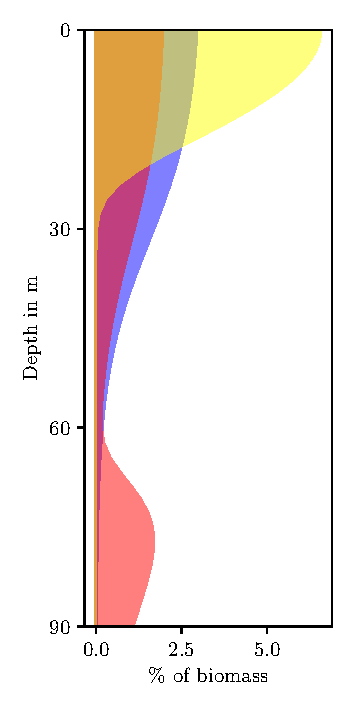
\includegraphics{plots/sketch_for_article.pdf}
 \end{centering}
 \label{fig:model_sketch}
 \caption{Sketch of model ecosystem, showing example distribution of resources, $(r(z,t)/R(t)$ \emph{(yellow)}, consumers ,$\phi_c$ \emph{(blue)} and predators, $\phi_p$ \emph{(red)}}
 \todo[inline]{Det er noget forvirrende at dette kun er ``example distribution''. Hvad skal læseren tage med sig fra denne figur?}
\end{figure}

Forage fish are visual predators, so their predation success is heavily light dependent. The available light decreases with depth in the water column, and varies with the time of day.
The light intensity $I$ at depth $z$ is approximately $I(z) = I_0\exp(-kz)$, and the light-dependent clearance rate of a predator is $\beta_{p,0}$.  However, even when there is no light available there is still a chance of catching a consumer if it is directly encountered,  so the clearance rate, $\beta_p(z,t)$, of forage fish never goes to 0 even at the middle of the night or at the deepest depths.
\begin{align*}
  \beta_p(z,t) = \beta_{p,0} \frac{I(z,t)}{1+I(z,t)} + \beta_{p,min}
\end{align*}


We model the light-levels at the surface via. the python package pvlib, using a simple Clear Sky model in Oresund between Denmark and Sweden. The light levels are given by the direct horizontal light intensity at the sea-surface, neglecting more complicated optic effects. The model takes the precipitable water $w_a$, and aerosol optical depth, $aod$. We model light decay throughout the water column as $\exp(-kz)$.


In contrast to forage fish, copepods are olfactory predators, and their clearance rate, $\beta_c$, is essentially independent of depth and light levels.
\begin{align*}
	\beta_c(z,t) &=  \beta_{c,0}
\end{align*}

The interactions between the consumer and resource are local, as are the interactions between a predator and a consumer. The local encounter rate between consumers and resources is given by $\beta_c(z,t)c(z,t)r(z,t)$, and the local encounter rate between predators and consumers is $\beta_p(z,t)c(z,t)p(z,t)$.

\subsubsection*{Population dynamics}

The resource cannot move actively, so its time dynamics are naturally specified locally. The growth of the resource is modeled with a logistic growth, with a loss from grazing by consumers and diffusion from the natural movement of the water. To simplify the model, we assume interactions can be described with a Type I functional response. %In natural environments, undersaturation of nutrients is the norm, \citep{}.


The total population growth of the consumer population is found by integrating the local grazing rate over the entire water column multiplied by a conversion efficiency $\epsilon$, subtracting the loss from predation. The growth of the predators is given by the predation rate integrated over the water column:
%Incorporating \Cref{eq:prob_dens} in \Cref{eq:population_growth}, we arrive at equations for the population dynamics governed by probability densities:
\begin{align}
	\dot{r} &= r(z,t)\pa{1-\frac{r(z,t)}{r_{max}(z)}} - \beta_c(z,t)\phi_c(z,t)C(t) r(z,t)  + k \partial_z^2 r(z,t)\\
	\dot{C} &= C(t)\left ( \int_0^{z_0} \varepsilon \beta_c(z,t)\phi_c(z,t)r(z,t) dz- P(t)\int_0^{z_0} \beta_p(z,t) \phi_c(z,t) \phi_p(z,t) dz - \mu_C \right ) \\
	\dot{P} &= P(t) \left ( C(t )\int_0^{z_0} \varepsilon \beta_p(z,t) \phi_c(z,t)\phi_p(z,t) dz - \mu_P \right )
  \label{eq:population_growth_prob_dens}
\end{align}
\todo[inline]{Kan vi ikke gøre disse ligninger lidt mere kompakte? Introducere optag som kan genbruges? Udelade nogle af argumenterne?}

\subsubsection*{Fitness proxies and optimal strategies}

The instantaneous fitness pr. capita of a forage fish $(F_p)$ or copepod $(F_c)$ is given by the total growth divided by the biomass. We arrive at the fitness by dividing the population growth rate \Cref{eq:population_growth_prob_dens} by the total populations, eliminating the terms $C(t), P(t)$ outside the parentheses in \Cref{eq:population_growth_prob_dens}.

\todo[inline]{Fitness er ikke det samme som specifikke vækstrater. }
\begin{align}
	F_c(\phi_c, \phi_p) &= \int_0^{z_0} \varepsilon \beta_c(z,t)\phi_c(z,t)r(z,t) dz\\ &- P(t)\int_0^{z_0} \beta_p(z,t) \phi_c(z,t) \phi_p(z,t)dz \\
	F_p(\phi_c, \phi_p) &=  C(t) \int_0^{z_0} \varepsilon \beta_p(z,t)\phi_c(z,t)\phi_p(z,t) dz
  \label{eq:fitness}
\end{align}
\todo[inline]{Når nu disse størrelser er indført, hvorfor så ikke bruge dem over det hele? Så ville mange formler være meget mere kompakte.}

At any instant, an organism seeks to find the strategy that maximizes its fitness. \todo{Her bør vi være mere præcise og henvise til det resultatet om ESS.} A strategy in our case is a probability distribution in the water column. The optimal strategy $\phi_c^*$ of a consumer depends on the strategy of the predators, and likewise for $\phi_p^*$ for the predators. Denoting the space of probability distributions on $[0,z_0]$ by $\mathbb{P}(0,z_0)$, this can be expressed as:
\begin{align*}
	\phi_c^*(z,t)(\phi_p) &= \argmax_{\phi_c \in \mathbb{P}(0,z_0)}  \int_0^{z_0} \varepsilon \beta_c(z,t)\phi_c(z,t)r(z,t) dz \\ &- P(t)\int_0^{z_0} \beta_p(z,t) \phi_c(z,t) \phi_p(z,t)dz  \\
	\phi_p^*(z,t)(\phi_c) &= \argmax_{\phi_p \in \mathbb{P}(0,z_0)}C(t) \int_0^{z_0} \varepsilon \beta_p(z,t)\phi_c(z,t)\phi_p(z,t) dz
\end{align*}
The Nash equilibrium of the instantaneous game is:
\begin{align}
  \label{eq:nash_equilibria}
	\phi_c^{*,NE} &=  \argmax_{\phi_c \in P(0,z_0)}  \int_0^{z_0} \varepsilon \beta_c(z,t)\phi_c(z,t)r(z,t) dz \\ &- P(t)\int_0^{z_0} \beta_p(z,t) \phi_c(z,t) \phi_p^{*,NE}(z,t) dz \\
	\phi_p^{*,NE} &=  \argmax_{\phi_p \in P(0,z_0)}C(t) \int_0^{z_0} \varepsilon \beta_p(z,t)\phi_c^{*,NE} \phi_p(z,t) dz
\end{align}
Since the fitness, \Cref{eq:fitness}, is a linear function of the strategies for the predator and prey we can apply the method \Cref{eq:lcp} to find the Nash equilibrium. Using this, we are able to solve the time-dynamics for the predator-prey system by a Euler scheme. The dynamics of the resource are more complicated due to the diffusion term, \Cref{eq:population_growth_prob_dens}. We solve the partial differential equation for the resource using the method of exponential time-differencing with a first-order approximation of the integral. Using exponential time-differencing guarantees a stable solution, though the system may be stiff, \cite{hochbruck2010exponential}

\subsubsection*{Model parametrization}
Following \citep{yodzis1992body}, we parametrize the clearance and loss rates in a metabolically scaled manner following Kleiber's law, \citep{yodzis1992body}, using scaling constants from \citep{kha_2019}. We use the default parameters in the clear-sky model, modeling a sequence of moonless nights. This is a bit of a simplification, but it should not have a great effect on our results. The North Sea\todo{Tidligere skrev du Øresund ... jeg foretrækker nu Nordsøen} is modeled with a rather high attenuation coefficient.


\begin{tabular}{l | l | l}
  Precipitable water & $w_a$ & 1 g $\cdot$ m$^{-3}$\\
  Aeorosol optical depth & $aod$ & 0.1 \\
  Light decay & $k$ & 0.1 m$^{-1}$\\
  Ocean depth & $z_0$ & 90 m \\
  Consumer mass & $m_c$ & 0.05 $g$ \\
  Predator mass & $m_p$ & 20 $g$ \\
  Consumer clearance rate & $\beta_c$ & 32 m$^{3}$ year$^{-1}$ \\
  Predator clearance rate & $\beta_p$ & 2800 m$^3$ year$^{-1}$ \\
  Consumer metabolic rate & $\mu_c$ & 0.24 g$^{3}$ year$^{-1}$ \\
  Predator metabolic rate & $\mu_p$ & 21 g$^3$ year$^{-1}$ \\
  Minimal attack rate & $\beta_0$ & $5 \cdot 10^{-3} \beta_p$ \\
  Phytoplankton growth & $\lambda$ & 100 year$^{-1}$ \\
  Phytoplankton max & $r_{max}$ & $10\mathcal{N}(0,6)$ g$\cdot$m$^{-1}$ \\
  Irrationality & $\sigma$ & 14 $m^2$ \\
  Diffusion rate & k & 500 m$^{2}$ year$^{-1}$
\end{tabular}

%%% Local Variables:
%%% mode: latex
%%% TeX-master: "main"
%%% End:


The following theorem is an adaption of \citep[Theorem 3.3]{} to our setting.

%whereby we show that the requirement of lower semicontinuity can be replace by the condition that the convex set is instead a convex cone. We largely follow their notational conventions.
\begin{lemma}\label{lem:technical}
	Let $K$ be the closed convex cone of a.e. positive functions in the real separable Hilbert space H=$L^2(X)^n$. Let $T:H \to H$ be a bounded linear operator such that $T(K) \subset K$, and assume that $T$ is coercive on $K$. If a sequence $w_n$ converges weakly to $w^*$, and $w_n - w^* \in K$ for all $n$, then $\liminf_{n} \ip{w_n}{T w_n} \geq \ip{w^*}{Tw^*}$.
\end{lemma}
\begin{proof}
	Defining the quadratic form $a(u,v)=\ip{u}{Tv}$, we can write:
	\begin{align*}
		\ip{(w_n-w^*)}{T(w_n-w^*)} \geq \alpha \norm{w_n-w^*} \geq 0
		\ip{w_n}{Tw_n}-\ip{w_n}{Tw^*}+\ip{w^*}{Tw_n} - \ip{w^*}{Tw^*} \geq 0
		\ip{w_n}{Tw_n} \geq \ip{w_n}{Tw^*}-\ip{w^*}{Tw_n} +\ip{w^*}{Tw^*}
	\end{align*}
	Then, taking $\liminf$ and using the weak continuity of $T$, we arrive at the desired.
\end{proof}
\begin{lemma



\begin{theorem}[Variational inequality formulation]
\label{thm:lcp_hilbert}
Let $C$ be the closed convex cone of a.e. positive functions in the real separable Hilbert space $H=L^2(X)^n$.

Let $S:H \to H$ be a bounded linear operator such that $S(C) \subset C$, and assume that $S$ is coercive on $K$. In addition, assume that $A:H \to R^n$ is weakly continous, positive, and coercive on $C$ and define the operator
\begin{align*}
	T = \begin{bmatrix} S & -A^* \\ A & 0 \end{bmatrix}
\end{align*}
Defining $K = C \osum \R_+^n$, for every $q$ in $W = \int(\{w \in X : \ip{w}{x} \geq 0\, \quad x  \in \int(ker(T+T^*) \cap K})$, the problem
\begin{equation}
	\ip{v-\overline{x}}{T\overline{x} + q} \geq 0, \quad \text{ for all } v\in K
\end{equation}
has a solution $\overline{x} \in K$.
\end{theorem}
\begin{proof}
	Assume $q \in W - T(K)$, then there exists $x_0$ such that
	\begin{equation}
		\label{eq:var_ineq}
		\ip{y}{q+Tx_0} > 0, \forall y \in \int(ker(T+T^*) \cap K
	\end{equation}
	Let $(\psi_n)_{n\in \N}$ be a sequence which is dense in $K$, with $\psi_0 = x_0$ and and define $X_n$ as the closure of the space spanned by the first $n$ elements, with corresponding projection $p_n: X \to X_n$, converging strongly to the identity on $X_{\infty} = \bigcup_{n \in \N} X_n$. Definining $K_n = X_n \cap K$, we have a natural system of inclusions of $K_n$ in $K_{n+1}$, defining $K^\infty = \bigcup_{\N} K_n \subset X_\infty$, we have $K^\infty = K$, and $p_n \to 1_K$ strongly. We can apply this system of projections to attain a system of finite-dimensional solutions to \Cref{eq:var_ineq}, by considering
\begin{equation}
	\ip{p_n y}{q+(p_nTp_n) x_0} \geq 0
\end{equation} 
by \Cref{thm:goeleven2}, each of the variational inequalities has a solution $u_n$. It remains to show that the sequence $u_n$ is uniformly bounded. Assume for contradiction that $u_n$ is unbounded, and consider the quantities $x_n = u_n/\norm{u_n}$ and $q_n = q / \norm{u_n}$. The sequence $x_n$ is clearly bounded, and since $u_n \in K_n$ for each $n$ and $K$ is assumed to be a convex cone, then $x_n \in K_n$ for each $n$ as well, therefore the weak limit of a subsequence $x_{n_k}$, $x^*$, is in $K$.  Considering the sequence $c_n = \ip{x_n}{x^*}$, this sequence has a monotone subsequence, corresponding to a subsequence of $x_n$ with the same weak limit. We briefly drop to considering only the part of the sequence which lies in $L^2(X)$, keeping the same notation for this part to ease the notational burden. T
Define the indicator function $1_{x^*}$ on the essential support of $x^*$. Since $X$ is a probability space, both $1_{x^*}$ and $1_{x^*}$ lie in $L^2(X)$.
Passing to this subsequence, consider the sequence $\ip{x-x_n}{1-1_{x^*}}$. As $x_n$ converges weakly to $x^*$, the sequence $\epsilon_n=(1-1_{x^*})x_n$ converges to 0. Defining $\tilde{x}_n =1_{x^*} x_n$, we can write $x_n = \tilde{x}_n + \epsilon_n$. Note that by construction $x^*-\tilde{x}_n \in C$. We now return to considering the full sequence.

Fix $v_0 \in K$, then there is an $n$ such that $v_0 \in K_n,\quad n \geq m$. For every $n \geq m$ we have the inequality
\begin{equation}
	\ip{-v_0/\norm{u_n}+x_n}{Tx_n+q_n} \leq 0
\end{equation}
Rewriting with $\tilde{x}_n, \epsilon_n$, we arrive at:
\begin{equation}
	\ip{-v_0/\norm{u_n}+\tilde{x}_n+\epsilon_n}{T(\tilde{x}_n+\epsilon_n)+q_n} \leq 0 \\
	\ip{-v_0/\norm{u_n}+\tilde{x}_n}{T\tilde{x}_n+q_n}+\ip{\epsilon_n}{T(\tilde{x}_n+\epsilon_n)+q_n}+\ip{-v_0/\norm{u_n}+\tilde{x}_n}{T\epsilon_n}
\end{equation}
Gathering all terms with $\epsilon_n$ in the sequence $k_n$, we can write:
\begin{equation}
	\ip{-v_0/\norm{u_n}+\tilde{x}_n}{T\tilde{x}_n+q_n}+k_n \leq 0
\end{equation}


By taking $\liminf$ and using \Cref{lem:technical} we arrive at $\ip{x^*}{Tx^*} \leq 0$, which implies that $\ip{x^*}{Tx^*}=0$, so $T^*x^* = - Tx^*$. By coercitivity of $S$ and $A$ we can choose a subsequence such that the limit $x^*$ is different from 0. For every $q$ in $K$ there exists an $x_0$ such that
\begin{align*}
	\ip{Tx_0+q}{v} > 0, \quad \forall v \in ker(T+T^*)\cap K
\end{align*}
In addition, by positivity of $T$, we can write up the inequality
\begin{align*}
	\ip{x_0}{Tx_n + q} - \ip{x_n}{q} \geq 0
\end{align*}
So $\ip{x_0}{Tx_n+q} \geq \ip{x_n}{q}$, taking limits gives $\ip{x_0}{Tx^*+q} \geq \ip{x^*}{q}$
Which is a contradiction to the previous inequality. Therefore the sequence $u_n$ must be uniformly bounded, and we can without loss of generality assume that $u_n$ is weakly convergent in an increasing fashion to $u^*$ as before.
Going back to the finite-dimensional case, we have the sequence of inequalities for any $x \in K$
\begin{equation}
	\ip{x - u_n}{q+Tu_n} \geq 0
\end{equation}
Splitting up, we arrive at
\begin{align*}
	\ip{x-u_n}{q}+\ip{x}{Tu_n}-\ip{u_n}{Tu_n} \geq 0
	\limsup_{n}(\ip{x-u_n}{q}+\ip{x}{Tu_n}) \geq \limsup_{n}\ip{u_n}{Tu_n} \geq 0
	\lim_{n} \ip{x-u_n}{q} + \lim_{n} \ip{x}{Tu_n} \geq \liminf{n} \ip{u_n}{T u_n} \geq \ip{u^*}{Tu^*}
	\ip{x-u^*}{q} + \ip{x}{Tu_n^*} \geq \ip{u^*}{Tu^*}
\end{align*}
showing that $\ip{x-u^*}{q}+\ip{x}{Tu^*}-\ip{u_n}{Tu^*} \geq 0$, thus there exists a solution to the problem. The solution set is bounded by an analogous argument to the boundedness of $u_n$,, and clearly closed, hence weakly compact.
\end{proof}\begin{corollary}[Linear complementarity problem]
  \label{cor:lcp_formulation}
  Let $H$ be a separable real Hilbert space, and define the closed convex cone $K=H^+$ consisting of positive elements. Assume $T$ satisfies the assumptions of \Cref{thm:lcp_hilbert}. Then the linear complementarity problem
  \begin{align*}
    &\ip{x}{Tx+q} = 0
    &Tx+q \in K, ~x \in K
  \end{align*}
  has a solution for $q \in H$ s.t. $\ip{q}{x} > 0$ where $x\in \ker(T+T^*) \cap K - T(K)$ .
\end{corollary}
\begin{proof}
  Set $v=0$ in \Cref{thm:lcp_hilbert}, then $\ip{\overline{x}}{T\overline{x} + q} \geq 0$. Inserting $v=2\overline{x}$, we arrive at
  $\ip{\overline{x}}{T\overline{x}+q}\leq 0$, so $\ip{x}{T\overline{x}+q} = 0$.
\end{proof}
\begin{definition}[N-player linear game] \label{def:lin_game}
  Let $(X,\mu)$ be a probability space, assuming for simplicity that $\mu$ is either discrete or  continuous. Assume that we have $N$ players with utility functions $U_i$ and strategies $\phi_i$. We assume that $\phi_i$ is a probability distribution, as well as lying in $L^2(X,\mu)$. Denote the space of feasible $\phi_i$ as $K$. The pairwise interactions are defined by a family of bounded linear operators $U_{ij}: L^2(X)\to L^2(X)$, ie. the payoff of player $i$ playing strategy $\phi_i$ against player $j$ with strategy $\phi_j$ is $\gammU_{ij}=\ip{\phi_i}{U_{ij} \phi_j}$. The total expected payoff $U_i(\phi^{-i})$ of player $i$ is given by
  \begin{equation}
    \ip{\phi_i}{\sum_{k=1}^N U_{ij} \phi_j}
  \end{equation}
\end{definition}
\begin{remark}
  Setting $X$ to be a finite set of points equipped with the normalized counting measure in \Cref{def:lin_game}, we recover the notion of a polymatrix game.
\end{remark}
\begin{definition}
  \label{def:total_payoff}
  Let $(X,\mu)$ be a probability space, $K$ a convex subset of $L^2(X)$, and $U_{ij}$ a finite collection of bounded operators $U_{ij}: K \to L^2(X)$. Define the total payoff operator $U:K^N \to K^N$ as:
  \begin{equation}
    U =
    \begin{bmatrix}
        0 & U_{1,2} & U_{1,3} &\dots & U_{1,N} \\
        U_{2,1} & 0 & U_{2,3} &\dots & U_{2,N} \\
        \vdots & \vdots & \vdots & \vdots & \vdots \\
        U_{N,1} & U_{N,2} & \dots & \dots & 0
    \end{bmatrix}
  \end{equation}
\end{definition}
We recall the generalized version of Farkas Lemma for future use:
\begin{lemma}
  \label{lem:farkas_lemma}
Given locally convex spaces $X$ and $Y$ and a strongly continuous linear map $A:X\to Y$, the following conditions are equivalent:
  \begin{align}
    Ax = b \text{ has a solution } x\in S
    A^* y^* \in cl(A(S^))* \Rightarrow \ip{y^*}{b} \geq 0
  \end{align}
	where $cl$ denotes the closure.
\end{lemma}
\begin{lemma}\label{lem:equiv_game}
	Given an $N$-player linear game $G = (U_{ij}, \phi_i, H)$ in the sense of \Cref{def:lin_game}, there exists an equivalent formulation of the game where all operators $U_{ij}$ are strictly positive on $H^{+}$.
\end{lemma}
\begin{proof}
	For any $\epsilon>0$, define the constant $c=\max_{ij} \norm{U_{ij}}+\epsilon$. Define the operators $\tilde{A}_{ij}$ through the bilinear forms $\ip{\cdot}{U_{ij}\cdot} + c\ip{\cdot}{1}\ip{1}{\cdot}$. Consider the game $\tilde{G}$ defined by this family. The payoff for any strategy pair $\phi_{i},~\phi_{j}$ has been changed by a constant. Therefore the set of Nash equilibria of $G$ and $\tilde{G}$ agree.
	For $x,y\in H^+$:
	\begin{align}
		-\norm{U_{ij}}\norm{x}\norm{y} &\leq \ip{x}{\tilde{A}y} \\
		\ip{x}{\tilde{A}_{ij}y} &= \ip{x}{U_{ij}y} + c\norm{x}_1\norm{y}_1
	\end{align}
	where $\norm{x}_1\norm{y}_1 \geq \norm{x}_2\norm{y}_2$, and by assumption $c+\norm{A} > 0$. Therefore
	\begin{equation}
		\ip{x}{U_{ij}y} + c\norm{x}_1\norm{y}_1 >0
	\end{equation}
\end{proof}
Our proof largely follows that of \citep{millerzucker}, adapted to a general setting and containing their result as a special case.
\begin{theorem} \label{thm:nash_eq}
  Let $(X,\mu)$ be a probability space, and assume that we have an $N$-player game in the sense of \Cref{def:lin_game}. Then the Nash equilibrium of \Cref{def:lin_game} can be found by solving a complementarity problem
  \begin{equation}
    &Mz+q=w \\
    &\ip{w}{z} = 0
    z \in K, w\in K
    \label{eq:complementarity_problem}
  \end{equation}
\end{theorem}
\begin{proof}
		We start by considering an equivalent game, where all payoffs are guaranteed strictly negative as in \Cref{lem:equiv_game}. To ease the notation, we still denote the payoff operators as $U_{ij}$, and the total payff operator as $U$.
    The requirements for a family $\Phi^*=(\phi_i^*)_{i=1}^N \in K^N$ to constitute a Nash equilibrium is: There is no other family $(\psi_i)_{i=1}^N$, such that
    \begin{equation}
        \ip{\phi_i^*}{\sum_{k=1}^N U_{ij} \phi_j^*} < \ip{\psi_i}{\sum_{k=1}^N U_{ij} \phi_j^*}
    \end{equation}
    for all $i\in \{1,\dots,N\}$.
    By linearity, this is equivalent to the condition that there is no point $\Phi \in K^n$ such that
    \begin{equation}
      \ip{\Phi^*-\Phi}{U \Phi^*} < 0
    \end{equation}
		Since $U$ is assumed strictly negative, we can slack the requirement that $\int \phi_i d\mu(x)=1$ to $\int \phi_i d\mu(x) \geq 1$, as a greater variation decreases the payoff. By defining the operator $A=-\osum_{i=1}^N \ip{1}{\cdot}$, and $q = (-1)^N$, we can express this requirement as
		\begin{equation}
			\label{eq:constraint}
			A \Phi \leq q, p \in K
		\end{equation}

    For $\Phi, \Phi^* \in K^n$, define the slack variable $d = \Phi - \Phi^*$. If $\phi_i^* = 0$ a.s., then $d_i \geq 0$ a.s., and $\int d_i d\mu(x) \geq 0$.

    Thus a vector $\Phi^* \in K^n$ is an equilibrium if and only if it satisfies \Cref{eq:constraint} and there is no $d \in L^2(X)^N$ such that
    \begin{equation}
      &\ip{-d}{U \Phi^*} < 0 \\
      \ip{\phi_i}{1} = 1 \Rightarrow -\int d_i \mu(x) \leq 0 \\
      \phi_i = 0 a.s. \text{ on } A\subset X \Rightarrow -d_i \leq 0  \text{ on } A\subset X
    \end{equation}s
    By applying \Cref{lem:farkas_lemma} to each condition in \Cref{eq:alternative_eq}, we see that \Cref{eq:alternative_eq} has no solution if and only if the system:
    \begin{equation}
      \begin{bmatrix} A^* & I_{N} \end{bmatrix}\begin{pmatrix} y \\ u \end{pmatrix}  = Up, y,u \in K
				\phi_i \geq 0 \text{ a.e on A } \Rightarrow u_i = 0 \text{ a.e on A }
				-\int \phi_i d\mu(x) < -1 \Rightarrow y_i=0
    \end{equation}
    has a solution.
		Defining the slack vector $v = q - Ap$, defining $z=p\osum u, w = y\osum v$, and
		\begin{align}
			M =\begin{bmatrix}
				R & -A^* \\
				A & 0
			\end{bmatrix}
		\end{align}
    We can formulate the problem of a finding a Nash equilibrium in the terms of a complementarity problem:
    \begin{equation}
      &Mz+q=w \\
      &\ip{w}{z} = 0
      z \in K, w\in K
    \end{equation}
    which has a solution by \Cref{cor:lcp_formulation}, giving existence of a Nash equilibrium.
  \end{enumerate}
\end{proof}
Having determined the existence of a Nash equilibrium in a general bilinear game in Hilbert space, we are left with one complication. The theorem we have just shown requires calculating the operator norm to find the Nash equilibrium, and this is a highly nontrivial task, so if we wish to solve the problem numerically we are left with a problem. However, the existence of a Nash equilibrium allows us to give a simpler statement, based on the KKT-conditions.
\begin{corollary}
	\label{cor:gen_nash_eq}
	Given a linear game \Cref{def:lin_game} and defining $U$ as in \Cref{def:total_payoff}, and defining
	\begin{equation}
	M=
		\begin{bmatrix}
			U & -A^* \\
			A & 0
		\end{bmatrix}
	\end{equation}
  A Nash equilibrium of \def{lin_game} can be determined by solving the problem:
	\begin{equation}
		&Mz+q=w \\
		&\ip{w}{z} = 0
		z \in K, w\in K
	\end{equation}
\end{corollary}
\begin{proof}
	By \Cref{thm:nash_eq}, the game defined in \Cref{def:lin_game} has a Nash equilibrium, so the system $(U_1(\Phi), \dots, U_{N})$ has a stationary point where $\phi \geq 0, \int \phi d\mu(x)= 1$, with slack variables $\psi_i$ satisfying $\ip{\psi_i}{\phi_i} = 0$ and $L(\Phi, \Psi) = 0$ where $L$ is the Lagrangian of the system by \citep[p. 286]{handbookofglobaloptimization}.
	The derivatives of the constraints are contained in the matrix $A$, and  $\nabla_i U_i = \sum_{j=1}^N U_{ij}\phi_j$, showing the desired.
\end{proof}
The two competing formulations of the Nash equilibrium have their own benefits. The formulation in \Cref{thm:nash_eq} lends itself directly to discretization, as by discretizing we immediately arrive in a setting where Lemkes algorithm applies since our matrix is copositive by construction. On the other hand, the problem as formulated in \Cref{cor:gen_nash_eq} allows for investigation of uniquness of Nash equilibria via. the methods of of variational inequalities, and can be used for abstract understanding of the equilibrium structure.

\begin{comment}
@article{craven1977generalizations,
  title={Generalizations of Farkas’ theorem},
  author={Craven, Bruce Desmond and Koliha, Jaromir Joseph},
  journal={SIAM Journal on Mathematical Analysis},
  volume={8},
  number={6},
  pages={983--997},
  year={1977},
  publisher={SIAM}
}
(5)
@article{glicksberg1952further,
  title={A further generalization of the Kakutani fixed point theorem, with application to Nash equilibrium points},
  author={Glicksberg, Irving L},
  journal={Proceedings of the American Mathematical Society},
  volume={3},
  number={1},
  pages={170--174},
  year={1952},
  publisher={JSTOR}
}
(2)


@article{goeleven1993solvability,
  title={On the solvability of noncoercive linear variational inequalities in separable Hilbert spaces},
  author={Goeleven, D},
  journal={Journal of Optimization Theory and Applications},
  volume={79},
  number={3},
  pages={493--511},
  year={1993},
  publisher={Springer}
}
\end{comment}

\section{Discussion}
%\subsection{What we found} %1 Paragraph
Our study of a Lotka-Volterra system with optimal behavior in the water column focuses on both the emergent behavior and population dynamics. The population dynamics were stabilized dramatically by the introduction of optimal behavior, and a slight seasonal dependence appeared. The short-term dynamics show a clear distinction between predator and consumer feeding modes, where prey feed during night while predators feed at dusk and dawn. By comparing the results for bounded rationality and unbounded rationality on the long and short time scales, we see two different pictures emerge. The behavior predicted by the two different models is similar, but still visibly different. Though the behavior is different, the difference becomes negligible at long-time scales. Of course the effect is a result of the relatively low bounded rationality we have chosen, which was chosen heuristically to smooth the distributions but not too much. The results illustrate the strength of our numerical approach to studying population games, and underline the importance of robust algorithms and discretization schemes.

\todo[inline]{Det med valget af ``bounded rationality'' bør uddybes - det er jo et kontinuum. Diskussionen her får det til at fremstå som om vi har valgt en \emph{a priori} oplagt værdi for niveauet af optimalitet. Så kan vi sige at vi har valgt niveauet af optimalitet sådan at de observerede fordelinger er forskellige fra perfekt optimalitet, mens den emergente populationsdynamik ikke er særligt påvirket?}

%\subsection{Interpretation of the findings and what they mean} %1-2 paragraphs
Our results illustrate the interplay between population dynamics, seasons, and behavior. Though light levels may be the same at two different times of the year, the migration patterns can differ radically due to the differences in \replaced{population abundances}{populations}. Bounded rationality appears to change the population dynamics imperceptibly compared to the results with perfect rationality. Behavior is probably not completely rational in reality, but the change from complete rationality to slightly  bounded rationality does not appear important for population dynamics. Assuming perfect rationality appears much more reasonable than full irrationality. At first sight, the intensity of predator-prey interactions at dawn and dusk seem to indicate that models need to be very fine-grained in time to capture population dynamics accurately. Zooming out to the long-term dynamics lends hope that the same dynamic could be captured with a rougher time-discretization.


%\subsection{Compare results to litterature} %2-3 paragraphs
In terms of the specific case of diel vertical migrations, large-scale geographical studies of the vertical migration indicate that population levels are a driving factor in the diel vertical migration \citep{klevjer2016large}, not just light. This corresponds to the predictions of our model, and shows the importance of modeling behavior explicitly. Our qualitative results on the seasonal variation of the vertical migration tentatively appear to correspond with empirical findings \citep{wang2014seasonal, beaugrand2001geographical, colebrook1979continuous}. This agreement is, it must be emphasized, qualitative in nature. If the model was tuned through empirical data to an ecosystem, perhaps it could be used to forecast seasonal changes in vertical migrations.

At the level of general population games, ocean population dynamics are driven by feeding at dusk and dawn \citep{benoit2014critical}, and our model provides a purely behavioral justification for this phenomenon. At the same time, our results show that the discontinuous feeding patterns gives rise to smooth long-term population dynamics. The population-level results support the usual approach of assuming perfect rationality in population games with interacting populations, though the behavior of each individual is most likely slightly sub-optimal \citep{hurly1999context}. Slight sub-optimality in the vertical distribution is not that important for overall population levels, so at the population level complete rationality provides almost no evolutionary benefit.

Bounded rationality as we introduce it is potentially testable, contrasting e.g. satisficing models, \citep{nonacs1993satisficing}. Empirical studies of copepod vertical migration patterns indicate that their distribution in the water column can be closely approximated by the smooth distribution we get from the model with bounded rationality \citep{hay1991zooplankton, visser2001observations}. Our model of bounded rationality passes the first test, but must be compared with more data.

\todo[inline]{Tydeliggør strukturen i diskussion. Måske vil at markere ``In terms of the specific case of diel vertical migrations,'' vs ``At the level of general population games,'' eller sådan noget.}
%Modelling population games as we do presents an example of a sequence of static mean-field games in continuous space, and, or interacting ideal free distributions \citep{cressman2004ideal, cressman2010ideal} if considering the steady-state.
If we look at the specific distributions we find, it is unclear if they satisfy the criteria for being multi-species ideal free distributions \citep{kvrivan2008ideal}, i.e. stable under best-response dynamics. The Nash equilibrium of the habitat selection game is unique \citep{verticalmigration}, and the distribution we find corresponds to that found in nature. In that sense, it is what would be expected of the ideal free distribution in a multi-species population game \citep{cressman2004ideal}.
\todo[inline]{Skal ovenstående måske ikke bare fjernes? Der er intet indhold...}


\todo{Er det følgende ikke et nyt afsnit?}
Interpreting strategies as distributions in space forms one of the two pillars of our model. This approach is heavily inspired by that of static mean field games \citep{lasry2007mean, blanchet2016optimal}, rather than classical evolutionary game-theory \cite{hofbauer1998evolutionary}. Thinking of the strategy of a population as a distribution rather being at specific locations turns out to be a powerful tool. Thinking in terms of distributions is what allows us to reformulate the game between predators and prey into a continuous polymatrix game, where the Nash equilibrium can theoretically be found. A theoretical reformulation of the population game cannot stand alone, leading to the second pillar of our project: The introduction of efficient numerical methods. A necessity for efficient numerical methods is stating the problem in a form that is easily solvable, and an efficient algorithm to solve that. Using a spectral scheme allows us to only use relatively few points for high precision, \citep{kopriva2009implementing}, giving half the problem statement. Together with a tractable method of solving polymtarix games \citep{miller1991copositive}, we have the full restatement of the problem. We then apply fast algorithms from modern optimization software \citep{Andersson2019, acary2019introduction} to solve the restated problem. This combination is fundamentally what allows us to consider a population game in both continuous time and space.
Overall, our approach is only possible due to an influence from the theory of mathematical optimization. Using insights from mean-field games motivates a change of perspective in how we view habitat selection. An efficient discretization and a good problem formulation allows us to solve the problem efficiently with modern numerical software.




%This focus on the distribution is what gives us the ability to consider continuous habitats, and allows the incorporation of complex spatial features in habitat selection games.





%\todo[inline]{Udmærkede elementer i diskussionen, men den bør struktureres klarere. Det specifikke omkring vertikale vandringer er står fint; .}
Our population model with the vertical migration shows that transient phenomena and continuous fitness gradients \citep{kawecki2004conceptual} are naturally at home in a continuous population game. Incorporating these features allows a more fine-grained biological analysis and greater predictive power in models of real-world systems than typical finite-patch models \citep{kvrivan2008ideal, sadowski2019predator}. Our focus has largely been on the interplay between temporal and spatial transients in the vertical migration. If one of these is averaged out, e.g. the time-varying habitat, the model can be adapted to find the equilibrium populations and distributions in inhomogeneous habitats. We have used our approach for a one-dimensional habitat, but it can readily be used to accommodate a two-dimensional habitat. More generally, our approach only depends on the bilinearity of the fitness proxy and the population-game setup.


%Our model can be used almost without modifications to model the population dynamics of complex aquatic communities \citep{pinti2019trophic}.  As an example, by using a Leslie matrix approach ontogenics could potentially be incorporated in the model. Doing so could potentially expand the model to handle life-cycle optimization.

%\subsection{Further work} %1 paragraph
A weakness of our model is that it does not incorporate satiation or other non-linear effects. Performing a multi-year simulation could also reveal interesting patterns, but doing so would complicate the model since it would need to take low-resource adaptations during winter into account. The distributions we arrive at with our model of bounded rationality for zooplankton qualitatively agree with observations, but to truly test our model of bounded rationality we need to make quantitative predictions and test then. Finally, it would be satisfying to find a general criterion to ensure that a continuous habitat selection game has a unique Nash equilibrium.


\section{Conclusion} %1 paragraph
Simulating the population dynamics of a predator-prey system through half a year reveal a complex interplay between seasons, behavior and population dynamics. Though our model is simple in nature, it can catch essential features of the seasonal dependence of the diel vertical migration. Though the primary trophic interactions happen abruptly and in a very short time frame when introducing optimal behavior, optimal behavior still serves to stabilize the system.
We show that it is possible to include bounded rationality in a systematic fashion, allowing it as a tuning parameter in future models. The usual assumption of perfect rationality seems to be reasonable for population dynamics, but bounded rationality appears to be better at predicting specific distributions.
These results are fundamentally only possible due to one of the major contributions of our approach, namely the introduction of efficient numerical methods for solving continuous population games. Whether to include behavior in a model or not reduces to a question of relevance to the model, not feasibility.
\todo[inline]{Et væsentligt element af bidraget mangler at blive nævnt: at beregningsmæssige metoder (Nash, diskretisering) muliggør at inddrage spil i populationsdynamik.}

%%% Local Variables:
%%% mode: latex
%%% TeX-master: "main"
%%% End:

%\input{conclusion.tex}


\bibliographystyle{alpha}
\bibliography{bibliography}

\end{document}
